\begin{figure}[h!]
	\centering
	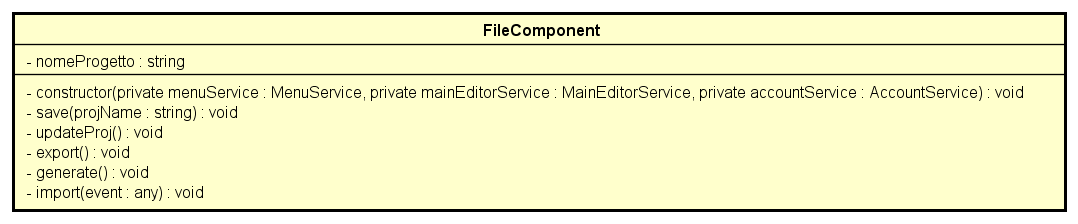
\includegraphics[scale=0.8]{res/sections/SpecificaFrontEnd/Components/Disegnetti/file.png}
	\caption{Diagramma della classe FileComponent}
\end{figure}

\begin{itemize}
	\item \textbf{Descrizione:}\\
	È il componente che descrive la voce \textit{File} del menu dell'editor.
	\item \textbf{Utilizzo:}\\
	
	\item \textbf{Attributi:}
		\begin{itemize}
			\item \emph{-nomeProgetto: string}\\
			Contiene il nome del progetto corrente
		\end{itemize}
	\item \textbf{Metodi:}
		\begin{itemize}
			\item \emph{-constructor(private menuService: MenuService,
    private mainEditorService: MainEditorService,
    private accountService: AccountService)}\\
    		Costruttore della classe\\
    		\textbf{Parametri:}
    		\begin{itemize}
    			\item \emph{menuService: MenuService}\\
    			Crea un istanziazione del MenuService
    			\item \emph{mainEditorService: MainEditorService}\\
    			Crea un istanziazione del MainEditorService
    			\item \emph{accountService: AccountService}\\
    			Crea un istanziazione di AccountService
    		\end{itemize}
    		\item \emph{-save(projName: string)}\\
    		Memorizza un progetto nel database\\
    		\textbf{Parametri:}
    		\begin{itemize}
    			\item \emph{projName: string}\\
    			Nome del progetto da memorizzare
    		\end{itemize}
    		\item \emph{-updateProj()}\\
    		Aggiorna un progetto esistente
    		\item \emph{-export()}\\
    		Esporta il progetto corrente
    		\item \emph{-generate()}\\
    		Genera il codice Java
    		\item \emph{-import(event: any)}\\
    		Importa un progetto esistente\\
    		\textbf{Parametri:}
    		\begin{itemize}
    			\item \emph{event: any}\\
    			Progetto da importare
    		\end{itemize}
		\end{itemize}
\end{itemize}